\section{Fourier变换下的运算}
\label{sec:fourier-operations}

有限维中，对称矩阵在特征向量基下变成对角矩阵，矩阵的作用只是把每个坐标乘一个数。平面波$e_\xi(x)=e^{2\pi\mathrm ix\cdot\xi}$对几种基本运算扮演同样的角色。平移$a$之后，
\[
e_\xi(x-a)=e^{-2\pi\mathrm ia\cdot\xi}\,e_\xi(x),
\]
求导之后，
\[
\partial_je_\xi=2\pi\mathrm i\xi_j\,e_\xi .
\]
所以每个平面波都是平移和求导的公共“特征向量”，而特征值是$\xi$的已知函数。这就是频率坐标好用的根本原因：这些运算在频率坐标下都是对角的。

这一说法只是启发。平面波不属于$L^1$，也不属于$L^2$，上面的“特征向量”并不在所讨论的空间里，所以每条规则都要用换元、分部积分或交换积分次序实际证明，而每一步都有前提。本节对每条规则先在$L^1(\mathbb R^d)$中给出证明，再说明它在什么条件下推广到$L^2$，所用的卷积与弱导数来自第~\ref{chap:smoothing-weak-derivatives}章。

\subsection{平移}
\label{sec:fourier-translation}

把函数整体移动$a\in\mathbb R^d$，记$(\tau_af)(x)=f(x-a)$。按上面的特征值，平移不应改变各频率成分的大小，只改变它们的相位。与之对偶的操作是乘以平面波，记$(M_bf)(x)=e^{2\pi\mathrm ib\cdot x}f(x)$，称为\term{调制}（modulation）。

\begin{theorem}[平移与调制]
\label{thm:fourier-translation}
设$f\in L^1(\mathbb R^d)$，$a,b\in\mathbb R^d$。则对每个$\xi$，
\begin{equation}
\widehat{\tau_af}(\xi)=e^{-2\pi\mathrm ia\cdot\xi}\,\widehat f(\xi),\qquad\widehat{M_bf}(\xi)=\widehat f(\xi-b).
\label{eq:fourier-translation}
\end{equation}
两式对$f\in L^2(\mathbb R^d)$在$L^2$意义下同样成立。
\end{theorem}

\begin{proof}
第一式作换元$x=y+a$：
\[
\int f(x-a)e^{-2\pi\mathrm ix\cdot\xi}\,\mathrm dx=\int f(y)e^{-2\pi\mathrm i(y+a)\cdot\xi}\,\mathrm dy=e^{-2\pi\mathrm ia\cdot\xi}\widehat f(\xi).
\]
第二式只需把两个指数合并成$e^{-2\pi\mathrm ix\cdot(\xi-b)}$。

对$L^2$，四个映射$f\mapsto\tau_af$、$f\mapsto M_bf$、乘以$e^{-2\pi\mathrm ia\cdot\xi}$、频率平移$b$都是$L^2$上的等距，$\mathcal F$也是。所以两边作为$f$的映射都连续，又在稠密子空间$L^1\cap L^2$上相等，因而在$L^2$上相等。
\end{proof}

两条规则方向相反，不能混淆。函数平移产生频率上的相位因子，频谱的大小$\lvert\widehat f\rvert$不变，完全看不出平移量；频率平移则来自函数上的相位因子。指数的符号取决于定义中的约定。周期情形有同样的规则，第$k$个坐标乘以$e^{-\mathrm ika}$，证明也是换元。

用$\mathbf 1_{[0,1]}=\tau_{1/2}B$作一个核对。平移规则与式~\eqref{eq:fourier-box}给出
\[
\widehat{\mathbf 1_{[0,1]}}(\xi)=e^{-\pi\mathrm i\xi}\,\frac{\sin\pi\xi}{\pi\xi}.
\]
直接积分得到$\frac{1-e^{-2\pi\mathrm i\xi}}{2\pi\mathrm i\xi}$，提出因子$e^{-\pi\mathrm i\xi}$后，
\[
\frac{1-e^{-2\pi\mathrm i\xi}}{2\pi\mathrm i\xi}=e^{-\pi\mathrm i\xi}\,\frac{e^{\pi\mathrm i\xi}-e^{-\pi\mathrm i\xi}}{2\pi\mathrm i\xi}=e^{-\pi\mathrm i\xi}\,\frac{\sin\pi\xi}{\pi\xi},
\]
两者一致。

\subsection{缩放}
\label{sec:fourier-scaling}

把自变量乘以$\lambda>1$，函数在空间中被压窄。频率的含义是单位长度内的圈数，压窄后同样的振荡出现在更短的长度上，频率应当按$\lambda$放大；同时积分区域缩小，幅度要乘以一个Jacobian因子。下面对一般的可逆线性变换推导这一点。

\begin{theorem}[线性变量替换]
\label{thm:fourier-scaling}
设$f\in L^1(\mathbb R^d)$，$\bm A$是$d\times d$可逆实矩阵。则
\begin{equation}
\widehat{f\circ\bm A}(\xi)=\frac1{\lvert\det\bm A\rvert}\,\widehat f\bigl(\bm A^{-\top}\xi\bigr).
\label{eq:fourier-linear-change}
\end{equation}
特别地，对实数$\lambda\neq0$，
\begin{equation}
\widehat{f(\lambda\,\cdot)}(\xi)=\lvert\lambda\rvert^{-d}\,\widehat f(\xi/\lambda).
\label{eq:fourier-scaling}
\end{equation}
\end{theorem}

\begin{proof}
作换元$y=\bm Ax$。Lebesgue测度在线性变换下乘以$\lvert\det\bm A\rvert$，即$\mathrm dx=\lvert\det\bm A\rvert^{-1}\mathrm dy$（第~\ref{chap:integration}章）。指数中的内积变成
\[
x\cdot\xi=(\bm A^{-1}y)\cdot\xi=y\cdot(\bm A^{-\top}\xi).
\]
代入定义，于是
\[
\int f(\bm Ax)e^{-2\pi\mathrm ix\cdot\xi}\,\mathrm dx=\frac1{\lvert\det\bm A\rvert}\int f(y)e^{-2\pi\mathrm iy\cdot\bm A^{-\top}\xi}\,\mathrm dy.
\]
取$\bm A=\lambda\bm I$，$\det\bm A=\lambda^d$，$\bm A^{-\top}\xi=\xi/\lambda$，就是第二式。
\end{proof}

公式中三个量各有来源。频率尺度$\xi/\lambda$说明：$\lambda>1$时原函数压窄，变换展宽。因子$\lvert\lambda\rvert^{-d}$是Jacobian，它随维数$d$改变；各坐标分别按$\lambda_1,\ldots,\lambda_d$缩放时，因子为$\prod_i\lvert\lambda_i\rvert^{-1}$，第$i$个频率坐标变为$\xi_i/\lambda_i$。转置逆$\bm A^{-\top}$说明频率按对偶方式变换：旋转在频域中仍是同一个旋转，剪切则不然。

图~\ref{fig:fourier-scaling}取$\lambda=1/2$。方框加宽一倍，式~\eqref{eq:fourier-scaling}给出
\[
\widehat{B(\cdot/2)}(\xi)=2\,\widehat B(2\xi)=\frac{\sin(2\pi\xi)}{\pi\xi},
\]
与上一节的直接计算一致。空间中变宽，频域中变窄；中央的高度翻倍，因为$\xi=0$处的值就是函数的积分，$\int B(x/2)\,\mathrm dx=2$。

\begin{BookInlineFigure}
  \centering
  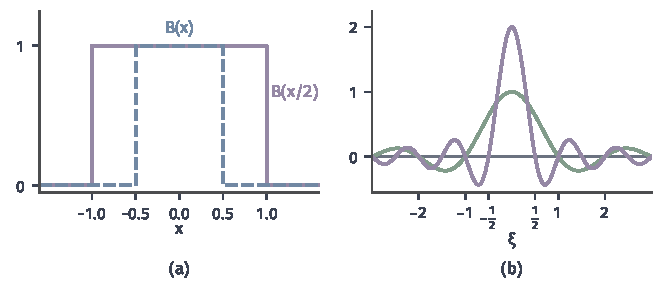
\includegraphics[width=112mm]{figures/04-spaces-measures-and-geometry/03-function-spaces/matplotlib/fourier-scaling/figure.pdf}
  \caption{缩放的对偶。(a)蓝色虚线为方框$B(x)$，紫色为加宽一倍的$B(x/2)$。(b)绿色为$\widehat B$，第一个零点在$\xi=\pm1$；紫色为$B(x/2)$的变换，第一个零点在$\xi=\pm\frac12$，中央高度为$2$。}
  \label{fig:fourier-scaling}
\end{BookInlineFigure}

Gauss核也可以检验。$G_t=t^{-d}G(\cdot/t)$对应$\lambda=1/t$，公式给出
\[
\widehat{G_t}(\xi)=t^{-d}\cdot t^d\,\widehat G(t\xi)=G(t\xi),
\]
正是反演证明中用到的等式。

在$L^2$中常用保持范数的伸缩
\[
D_\lambda f=\lvert\lambda\rvert^{d/2}f(\lambda\,\cdot).
\]
式~\eqref{eq:fourier-scaling}给出$\widehat{D_\lambda f}=D_{1/\lambda}\widehat f$。两边都是$L^2$上的等距，在$L^1\cap L^2$上相等，所以在$L^2$上相等。这一归一化把Jacobian因子平分到两侧，第~\ref{chap:wavelet-transform}章的小波伸缩采用同样的写法。

\subsection{微分}
\label{sec:fourier-differentiation}

周期情形的分部积分给出$\widehat{f'}(k)=\mathrm ik\widehat f(k)$，边界项因周期性抵消。全空间上没有周期，边界项能否消失取决于函数在远处的行为；在函数不可导的点，还要借助弱导数。下面先处理边界项自动消失的情形，再处理一般情形。

\paragraph{光滑紧支撑函数}

设$f$连续可微且支撑紧。固定其余坐标，在一个包含支撑的有界区间上对$x_j$分部积分，边界项为零，得到
\[
\int\partial_jf(x)\,e^{-2\pi\mathrm ix\cdot\xi}\,\mathrm dx_j=-\int f(x)\,\partial_j\bigl(e^{-2\pi\mathrm ix\cdot\xi}\bigr)\,\mathrm dx_j.
\]
指数对$x_j$求导带下来因子$-2\pi\mathrm i\xi_j$，所以
\[
\int\partial_jf(x)\,e^{-2\pi\mathrm ix\cdot\xi}\,\mathrm dx_j=2\pi\mathrm i\xi_j\int f(x)e^{-2\pi\mathrm ix\cdot\xi}\,\mathrm dx_j.
\]
再对其余坐标积分（Fubini定理），得到
\[
\widehat{\partial_jf}(\xi)=2\pi\mathrm i\xi_j\,\widehat f(\xi).
\]
求导在频域中变成乘以$2\pi\mathrm i\xi_j$，与开头的特征值一致。

\paragraph{弱导数可积的情形}

一般的可积函数没有紧支撑，也未必处处可导。第~\ref{chap:smoothing-weak-derivatives}章用测试恒等式定义了弱导数：若局部可积函数$g$对所有$\varphi\in C_c^\infty(\mathbb R^d)$满足$\int f\,\partial_j\varphi=-\int g\,\varphi$，就称$g$为$f$的弱导数$\partial_jf$。要把这个恒等式用于$e^{-2\pi\mathrm ix\cdot\xi}$，需要先把它截断成紧支撑函数，再让截断半径趋于无穷，并控制截断边缘产生的项。

\begin{theorem}[微分规则]
\label{thm:fourier-derivative}
设$f\in L^1(\mathbb R^d)$，且$f$关于$x_j$的弱导数$\partial_jf$存在并属于$L^1(\mathbb R^d)$。则对每个$\xi\in\mathbb R^d$，
\begin{equation}
\widehat{\partial_jf}(\xi)=2\pi\mathrm i\xi_j\,\widehat f(\xi).
\label{eq:fourier-derivative}
\end{equation}
\end{theorem}

\begin{proof}
取光滑函数$\chi$，满足$0\leq\chi\leq1$，在$\lvert x\rvert\leq1$上等于$1$，在$\lvert x\rvert\geq2$上等于$0$；这样的截断函数由第~\ref{chap:smoothing-weak-derivatives}章的磨光构造得到。对$R>0$令
\[
\varphi_R(x)=\chi(x/R)\,e^{-2\pi\mathrm ix\cdot\xi},
\]
它的实部与虚部都是测试函数，所以测试恒等式对$\varphi_R$成立。按乘积求导，
\[
\partial_j\varphi_R(x)=\Bigl[\frac1R(\partial_j\chi)(x/R)-2\pi\mathrm i\xi_j\chi(x/R)\Bigr]e^{-2\pi\mathrm ix\cdot\xi}.
\]
代入测试恒等式，得到
\[
\begin{aligned}
\int\partial_jf(x)\chi(x/R)e^{-2\pi\mathrm ix\cdot\xi}\,\mathrm dx
={}&-\frac1R\int f(x)(\partial_j\chi)(x/R)e^{-2\pi\mathrm ix\cdot\xi}\,\mathrm dx\\
&+2\pi\mathrm i\xi_j\int f(x)\chi(x/R)e^{-2\pi\mathrm ix\cdot\xi}\,\mathrm dx .
\end{aligned}
\]
令$R\to\infty$。左边与右边第二项的被积函数分别被$\lvert\partial_jf\rvert$与$\lvert f\rvert$控制，且$\chi(x/R)\to1$，由控制收敛定理，它们分别趋于$\widehat{\partial_jf}(\xi)$与$2\pi\mathrm i\xi_j\widehat f(\xi)$。右边第一项是截断边缘的贡献，其模不超过
\[
\frac1R\sup\lvert\partial_j\chi\rvert\,\lVert f\rVert_1\to0.
\]
\end{proof}

证明中$f\in L^1$承担了控制边缘项的任务：截断函数的导数只有$1/R$大小，乘上可积的$f$后整体趋于零。这里没有要求$f$在远处逐点趋于零。

\paragraph{光滑性与衰减}

微分规则把光滑性转换为高频衰减。由定理~\ref{thm:fourier-l1-properties}，
\[
2\pi\lvert\xi_j\rvert\,\lvert\widehat f(\xi)\rvert=\lvert\widehat{\partial_jf}(\xi)\rvert\leq\lVert\partial_jf\rVert_1 .
\]
若各阶弱导数$\partial^\alpha f$（$\lvert\alpha\rvert\leq m$）都可积，逐次使用规则，得到
\[
\widehat{\partial^\alpha f}(\xi)=(2\pi\mathrm i\xi)^\alpha\,\widehat f(\xi),\qquad
(2\pi\mathrm i\xi)^\alpha=\prod_j(2\pi\mathrm i\xi_j)^{\alpha_j},
\]
所以$\lvert\widehat f(\xi)\rvert$按$\lvert\xi\rvert^{-m}$衰减。

对偶地，原函数在远处衰减得快，变换就光滑。若$f$与$x_jf$都可积，在积分号下对$\xi_j$求导（被积函数的导数被$2\pi\lvert x_jf\rvert$控制），得到
\[
\partial_{\xi_j}\widehat f=\widehat{-2\pi\mathrm ix_jf}.
\]

用双边指数核对。$f(x)=e^{-\lvert x\rvert}$在$0$处不可导，但有可积的弱导数$-\operatorname{sgn}(x)e^{-\lvert x\rvert}$。把弱导数的变换分成两段积分，得到
\[
-\frac1{1+2\pi\mathrm i\xi}+\frac1{1-2\pi\mathrm i\xi}=\frac{4\pi\mathrm i\xi}{1+4\pi^2\xi^2}.
\]
由式~\eqref{eq:fourier-double-exponential}，这恰好等于$2\pi\mathrm i\xi\,\widehat f(\xi)$，与定理一致。

方框$B$不满足定理的条件。形式地计算，
\[
2\pi\mathrm i\xi\,\widehat B(\xi)=2\mathrm i\sin(\pi\xi)=e^{\pi\mathrm i\xi}-e^{-\pi\mathrm i\xi}.
\]
它不随$\lvert\xi\rvert\to\infty$趋于零，由Riemann--Lebesgue引理不可能是可积函数的变换。它对应的是在$x=-1/2$与$x=1/2$处的两个符号相反的点质量，这正是跳跃函数的导数不能由局部可积函数表示的情形，超出了本节$L^1$的框架。

$L^2$函数的弱导数有对应的频域刻画：$f$与$\partial_jf$都属于$L^2$时，式~\eqref{eq:fourier-derivative}在$L^2$意义下成立。它是第~\ref{chap:sobolev-spaces}章用频率权刻画Sobolev空间的出发点，证明也留到那里。

\subsection{卷积}
\label{sec:fourier-convolution}

第~\ref{chap:smoothing-weak-derivatives}章对$f,g\in L^1(\mathbb R^d)$定义了卷积$(f*g)(x)=\int f(x-y)g(y)\,\mathrm dy$，证明它几乎处处有定义，并且
\[
\lVert f*g\rVert_1\leq\lVert f\rVert_1\lVert g\rVert_1.
\]

卷积是平移的加权叠加：
\[
f*g=\int g(y)\,\tau_yf\,\mathrm dy.
\]
平移在频域中是乘以相位因子，叠加之后应当得到$\widehat f$乘以$g$的相位加权和，也就是$\widehat f\,\widehat g$。在有限维的类比中，这说明卷积算子也在频率坐标下对角，第$\xi$个对角元就是$\widehat g(\xi)$。

\begin{theorem}[卷积规则]
\label{thm:fourier-convolution}
若$f,g\in L^1(\mathbb R^d)$，则对每个$\xi$，
\begin{equation}
\widehat{f*g}(\xi)=\widehat f(\xi)\,\widehat g(\xi).
\label{eq:fourier-convolution}
\end{equation}
\end{theorem}

\begin{proof}
先确认可以交换积分次序：
\[
\int\!\!\int\lvert f(x-y)\rvert\,\lvert g(y)\rvert\,\mathrm dx\,\mathrm dy=\lVert f\rVert_1\lVert g\rVert_1<\infty.
\]
由Fubini定理交换次序，再对内层换元$z=x-y$，得到
\[
\begin{aligned}
\widehat{f*g}(\xi)&=\int g(y)\Bigl(\int f(x-y)e^{-2\pi\mathrm ix\cdot\xi}\,\mathrm dx\Bigr)\mathrm dy\\
&=\int g(y)e^{-2\pi\mathrm iy\cdot\xi}\,\mathrm dy\cdot\int f(z)e^{-2\pi\mathrm iz\cdot\xi}\,\mathrm dz .
\end{aligned}
\]
\end{proof}

方框与自身的卷积是三角形。$(B*B)(x)$等于区间$[-1/2,1/2]$与$[x-1/2,x+1/2]$的重叠长度，所以
\[
(B*B)(x)=\Lambda(x)=\max\{0,1-\lvert x\rvert\}.
\]
图~\ref{fig:fourier-convolution-triangle}(a)画的是$x=0.4$的情形，重叠长度为$0.6$，正是(b)中$\Lambda(0.4)$的值。

卷积规则给出$\Lambda$的变换：
\[
\widehat\Lambda(\xi)=\Bigl(\frac{\sin\pi\xi}{\pi\xi}\Bigr)^2.
\]
它按$\xi^{-2}$衰减，是可积的，而$\Lambda$连续，所以由定理~\ref{thm:fourier-l1-inversion}，反演在每一点成立。在$x=0$处读出
\[
\int_{\mathbb R}\Bigl(\frac{\sin\pi\xi}{\pi\xi}\Bigr)^2\,\mathrm d\xi=\Lambda(0)=1,
\]
与上一节由能量关系算出的值一致。卷积使跳跃变成尖点，频域中的衰减也从$\xi^{-1}$加快到$\xi^{-2}$，图~\ref{fig:fourier-convolution-triangle}(c)中实线的旁瓣明显更小。

\begin{BookInlineFigure}
  \centering
  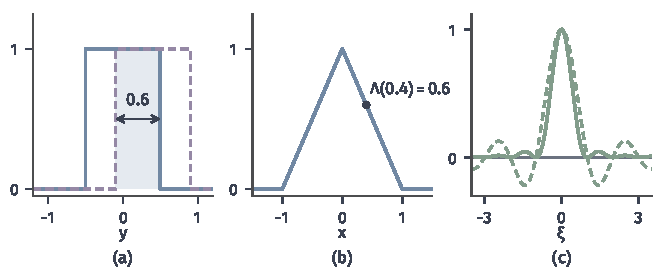
\includegraphics[width=112mm]{figures/04-spaces-measures-and-geometry/03-function-spaces/matplotlib/fourier-convolution-triangle/figure.pdf}
  \caption{方框的自卷积。(a)蓝色为$B(y)$，紫色虚线为$B(x-y)$（$x=0.4$），浅蓝色区域为重叠部分，长度$0.6$。(b)$\Lambda=B*B$，黑点对应(a)的$x$。(c)绿色虚线为$\widehat B$，绿色实线为$\widehat\Lambda=\widehat B^{\,2}$。}
  \label{fig:fourier-convolution-triangle}
\end{BookInlineFigure}

\paragraph{推广到$L^2$}

推广时要分别确认输入在哪个空间、卷积落在哪个空间、等式在什么意义下成立。

第一种情形是$f\in L^1$、$g\in L^2$。由Cauchy--Schwarz不等式，
\[
\lvert(f*g)(x)\rvert^2\leq\int\lvert f(x-y)\rvert\,\mathrm dy\cdot\int\lvert f(x-y)\rvert\,\lvert g(y)\rvert^2\,\mathrm dy.
\]
对$x$积分，得到
\[
\lVert f*g\rVert_2\leq\lVert f\rVert_1\lVert g\rVert_2,
\]
所以卷积落在$L^2$中，并且连续地依赖$g$。

此时等式$\widehat{f*g}=\widehat f\,\widehat g$在$L^2$中成立。当$g\in L^1\cap L^2$时它由定理~\ref{thm:fourier-convolution}给出。左边是$g$的连续映射，右边是乘以有界函数$\widehat f$，也连续。两边在稠密子空间上相等，所以在整个$L^2$上相等。

第二种情形是$f,g\in L^2$。此时$(f*g)(x)$对每个$x$都有定义，模不超过$\lVert f\rVert_2\lVert g\rVert_2$，由$L^2$平移连续性它还是连续函数；但它一般不属于$L^1$，也不必属于$L^2$。另一方面，$\widehat f\widehat g$作为两个$L^2$函数的乘积是可积的。因此正确的对应是逆变换，而不是$L^2$中的变换等式：
\begin{equation}
(f*g)(x)=\int_{\mathbb R^d}\widehat f(\xi)\,\widehat g(\xi)\,e^{2\pi\mathrm ix\cdot\xi}\,\mathrm d\xi\qquad\text{对每个}\ x .
\label{eq:fourier-l2-convolution}
\end{equation}

证明用Parseval关系。令$h_x(y)=f(x-y)$，则
\[
(f*g)(x)=\int h_x\,g=\langle\overline{h_x},g\rangle.
\]
由平移、反射规则，
\[
\widehat{h_x}(\xi)=e^{-2\pi\mathrm ix\cdot\xi}\widehat f(-\xi).
\]
再由共轭的规则
\[
\widehat{\overline u}(\xi)=\overline{\widehat u(-\xi)}
\]
（对$L^1$函数直接验证，再延拓到$L^2$），得到
\[
\widehat{\overline{h_x}}(\xi)=\overline{e^{2\pi\mathrm ix\cdot\xi}\widehat f(\xi)}.
\]
代入式~\eqref{eq:fourier-l2-parseval}，共轭抵消，即得式~\eqref{eq:fourier-l2-convolution}。

例如$f=g=s$时，$\widehat f\widehat g=B\cdot B=B$，式~\eqref{eq:fourier-l2-convolution}给出$s*s=s$，它平方可积却不可积。

这三种情形研究的都是Fourier变换怎样把卷积这一运算转为乘法。把卷积看作对信号的作用，讨论哪些频率被保留、哪些被削弱，属于滤波问题，在\BookChapterRef{chap:signal-systems}{卷九“信号系统”章}研究。
